\documentclass[11pt,letterpaper]{article}
\PassOptionsToPackage{hyphens}{url}
\usepackage[margin=.83in,top=.8in,bottom=.8in,headheight=15pt]{geometry}
\usepackage[T1]{fontenc}
\usepackage{lmodern,amsmath,amssymb,mathtools,bm,booktabs,array,graphicx,tikz}
\usetikzlibrary{arrows.meta,positioning,calc,decorations.pathreplacing,patterns}
\definecolor{ink}{HTML}{17344D}\definecolor{accent}{HTML}{087E8B}\definecolor{pale}{HTML}{EDF5F5}\definecolor{gold}{HTML}{AD6B19}
\providecommand{\dd}{\,\mathrm{d}}\providecommand{\R}{\mathbb{R}}
\providecommand{\E}{\mathbb{E}}\providecommand{\Var}{\operatorname{Var}}
\providecommand{\Cov}{\operatorname{Cov}}\providecommand{\diag}{\operatorname{diag}}
\providecommand{\norm}[1]{\left\lVert#1\right\rVert}
\providecommand{\abs}[1]{\left|#1\right|}
\usepackage{microtype,hyperref,fancyhdr,enumitem,amsthm,sectsty,needspace}
\allsectionsfont{\raggedright}
\hypersetup{colorlinks=true,linkcolor=ink,urlcolor=accent,pdfauthor={Zan Ahmad},pdftitle={Rigid alignment and arclength representations of closed curves / Lecture notes}}
\setlength{\parindent}{0pt}\setlength{\parskip}{6pt}\linespread{1.07}
\setlist{itemsep=3pt,topsep=4pt,leftmargin=*}
\emergencystretch=2em\clubpenalty=10000\widowpenalty=10000
\pagestyle{fancy}\fancyhf{}\fancyhead[L]{\small Computational Cardiology}\fancyhead[R]{\small Lecture 13}
\fancyfoot[L]{\footnotesize Zan Ahmad}\fancyfoot[R]{\footnotesize\thepage}\renewcommand{\headrulewidth}{.3pt}
\newtheorem{proposition}{Proposition}\newtheorem{theorem}{Theorem}\newtheorem{lemma}{Lemma}
\theoremstyle{definition}\newtheorem{definition}{Definition}\newtheorem{example}{Example}
\numberwithin{equation}{section}
\begin{document}
{\small\scshape Computational Cardiology\hfill Lecture 13}\par\medskip
{\raggedright\hyphenpenalty=10000\exhyphenpenalty=10000\LARGE\bfseries\color{ink} Rigid alignment and arclength representations of closed curves\par}\medskip
{\small Lecture notes}\par\bigskip
A comparison of contours depends on coordinates, point order and the transformations regarded as irrelevant. We retain physical size and handedness, remove translation and proper rotation, and derive the corresponding least-squares fit. Arclength resampling addresses a separate issue: how the boundary is represented by ordered vertices.

\section{Ordered polygonal representations}
\hypertarget{note-ordered-polygonal-representations}{}\label{note:ordered-polygonal-representations}
{\small \href{slides.html\#frame=a-cyclic-polygon-in-physical-coordinates\&step=1}{Slides for this section}}\par
An image, a contour, a point cloud and a surface mesh carry different information. A contour records an ordered boundary in a plane. A point cloud may lose the order needed to identify neighboring locations. A surface mesh adds connectivity in three dimensions, while a binary image retains a sampling grid and an inside/outside decision. Choosing a representation is already a scientific decision: it specifies which changes can be observed and which have been discarded. For an anatomical question, the acquisition plane, segmentation rule and units would also need documentation.

Here the object is a synthetic closed planar contour, stored as an n by 2 array of coordinates in millimetres. Row j is a point, the next row is its neighbor, and the last point connects back to the first. The first point is not duplicated at the end. That convention avoids giving one location extra weight in averages. The contour is generated from a smooth formula, but the stored polygon contains only straight segments between sampled vertices. Its shape is invented for this exercise and carries no diagnosis.

The synthetic generator uses a radial function with a small threefold cosine term and a twofold sine term, then compresses the y coordinate by a factor of 0.7. The angle is in radians and the radius scale is 12 mm. The formula creates an asymmetric test contour rather than a fitted anatomical model.

\[
\begin{aligned}r(\theta)&=12[1+0.16\cos(3\theta)+0.07\sin(2\theta)]\;\mathrm{mm}\\(x,y)&=(r\cos\theta,0.7r\sin\theta)\end{aligned}
\]
The angle runs once around the circle. The stored polygon samples this analytic curve; no measured anatomy is used.

A closed polygon is a cyclic sequence $X=(x_0,\ldots,x_{n-1})$ with the additional edge $(x_{n-1},x_0)$. The sequence contains adjacency information that an unordered point cloud does not. Duplicating $x_0$ as a final row would also duplicate its weight in the vertex mean and RMS discrepancy.
\Needspace{10\baselineskip}

\section{Physical size and pose invariance}
\hypertarget{note-physical-size-and-pose-invariance}{}\label{note:physical-size-and-pose-invariance}
{\small \href{slides.html\#frame=corresponding-point-rms\&step=1}{Slides for this section}}\par
Two arrays can describe the same object in different coordinate frames. Translation moves every point by the same vector. A proper rotation changes orientation while preserving lengths and handedness. These operations describe pose in this lesson. A uniform scale change alters every physical length and is deliberately retained. Reflection is also retained: allowing a mirror transformation would remove handedness, which may matter to a later anatomical question. The set of transformations we remove must be stated before looking at a desired result.

Centering subtracts the arithmetic mean of the stored vertices. It removes translation and makes the rotation calculation easier. This mean is a vertex centroid, not automatically an area centroid or center of mass. Dense sampling along one boundary region gives that region more influence. Two samplings of the same smooth curve can consequently have different vertex centroids. When equal arclength sampling is chosen, each boundary interval receives approximately equal influence, but the area inside the contour is still not being averaged.

The root-mean-square discrepancy pairs row j in one array with row j in the other. Square each two-dimensional displacement length, average those squared lengths, then take the square root. The result has units of millimetres. Division by n makes it an average per point, but it does not correct a poor correspondence or biased sampling. Always inspect the paired curves as well as the single number. A small average can hide a localized mismatch that deserves a separate maximum or regional diagnostic.

\[
d_{\rm RMS}(X,Y)=\sqrt{\frac1n\sum_{j=0}^{n-1}\|x_j-y_j\|^2}
\]
Coordinates and RMS are in mm; squared lengths are in mm\ensuremath{^{2}}. The same index j must refer to the intended corresponding location.

Translation and proper rotation form the rigid-motion action $Y\mapsto YR+\boldsymbol1t$, with $R\in SO(2)$. A scale factor is deliberately absent. The centered arrays $X_c=X-\boldsymbol1\bar x$ and $Y_c=Y-\boldsymbol1\bar y$ remove translation, leaving a rotation problem on corresponding rows.

\paragraph{Calculation.} A three-point landmark set in millimetres is X = [(0,0),(3,0),(0,3)]. Let Y = X + (2,\ensuremath{-}1). What changes under centering?

The vertex mean of X is (1,1); the mean of Y is (3,0).

Every raw displacement has squared length 2\ensuremath{^{2}} + (\ensuremath{-}1)\ensuremath{^{2}} = 5 mm\ensuremath{^{2}}, so raw RMS is sqrt(5) mm.

Subtracting each set's own mean yields identical centered arrays.

Translation accounts for the entire discrepancy; centered RMS is zero. These are landmark averages, not an area-centroid calculation.
\Needspace{10\baselineskip}

\section{The proper orthogonal Procrustes problem}
\hypertarget{note-the-proper-orthogonal-procrustes-problem}{}\label{note:the-proper-orthogonal-procrustes-problem}
{\small \href{slides.html\#frame=expand-the-least-squares-objective\&step=1}{Slides for this section}}\par
With correspondence fixed, choose the proper rotation and translation that minimize RMS. The supplied routine centers both arrays, forms a 2 by 2 cross-product matrix, and uses a singular-value decomposition to find the best rotation. In the implementation coordinates are row vectors: an aligned point is y multiplied on the right by R, then translated. Row-vector rotation signs differ from a familiar column-vector convention.

The determinant condition matters. An orthogonal matrix preserves lengths, but determinant minus one permits a reflection. The routine corrects the singular-value construction so that the determinant is plus one. Its output is therefore a proper rotation, with no hidden scale normalization. The diagnostic includes the rotation determinant and the residual in millimetres. For an exactly rotated and translated copy with matching rows, the residual should be close to floating-point roundoff. For a larger or locally deformed curve it should generally remain positive.

A unique numerical rotation is not guaranteed for every dataset. Repeated shapes or special symmetric configurations can admit equally good matches, and zero-spread point sets contain no orientation information. The companion rejects zero spread and reports a minimizing transformation for the other allowed inputs. Its success establishes an optimum for the stated fixed pairs, not anatomical correctness. A visually convincing overlay can result from comparing the wrong structures; data provenance and correspondence remain separate evidence.

\[
\min_{R,t}\;\frac1n\sum_j\|x_j-(y_jR+t)\|^2,\qquad R^TR=I,\quad\det R=1
\]
R is a 2 by 2 dimensionless rotation; t is a two-component translation in mm. Scale and reflection are excluded.

For fixed $R$, the minimizing translation is $t=\bar x-\bar yR$. Expanding the remaining squared Frobenius norm gives
\[
 \|X_c-Y_cR\|_F^2=\|X_c\|_F^2+\|Y_c\|_F^2
 -2\operatorname{tr}(R^{\mathsf T}Y_c^{\mathsf T}X_c).
\]
Let $Y_c^{\mathsf T}X_c=U\Sigma V^{\mathsf T}$. The proper-rotation solution is
\[
 R=U\operatorname{diag}\bigl(1,\det(UV^{\mathsf T})\bigr)V^{\mathsf T}.
\]
The determinant correction prevents a reflection. This derivation uses row vectors and aligns $Y$ to $X$; transposing conventions without changing the formula would reverse the interpretation.
\Needspace{10\baselineskip}

\begin{center}\begin{minipage}{.98\linewidth}\centering
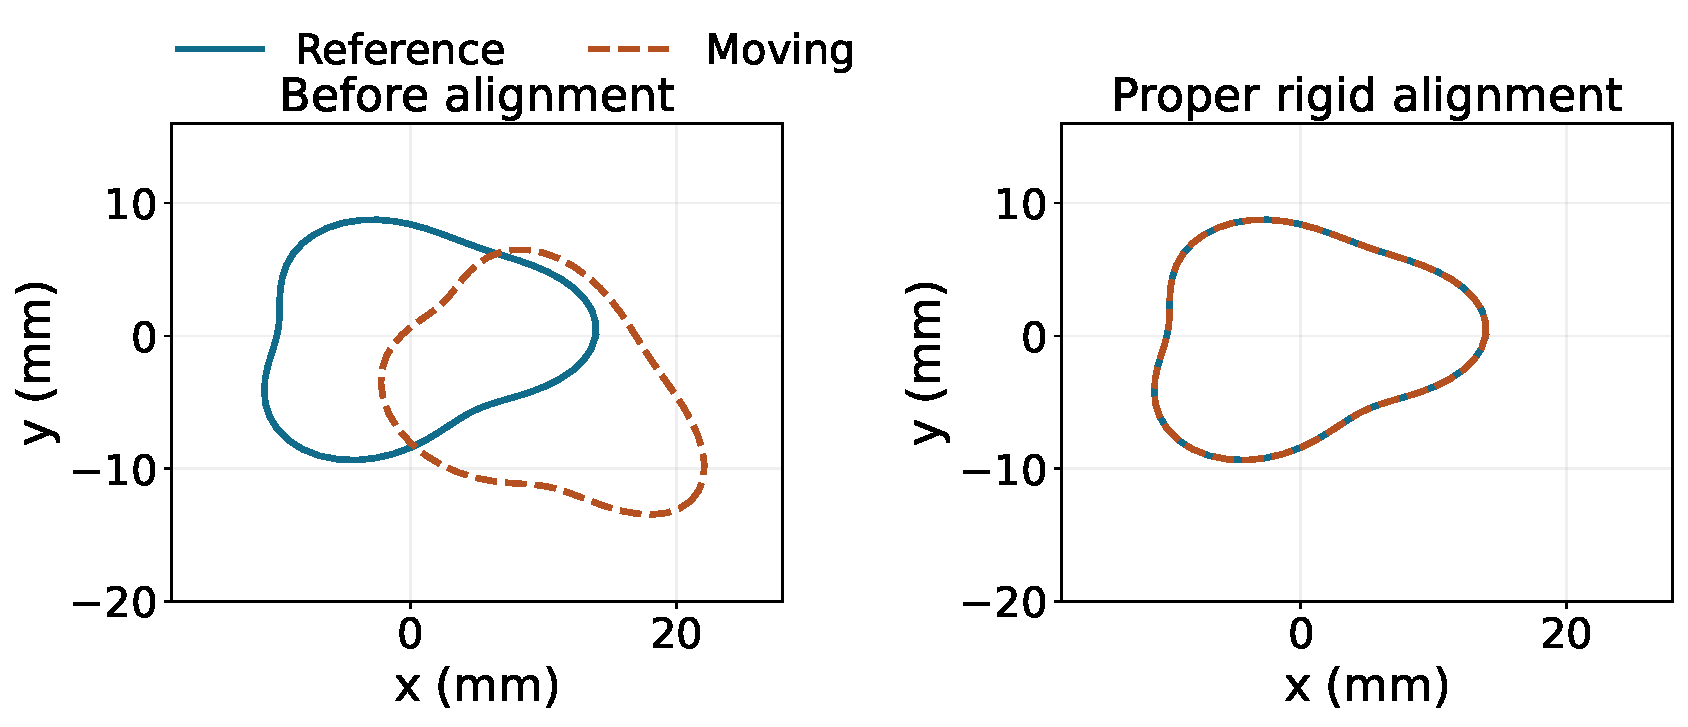
\includegraphics[width=.96\linewidth,height=.57\textheight,keepaspectratio]{pose-alignment.pdf}\par\smallskip
{\small Original synthetic contours in mm. Solid reference and dashed moving contour use identical axis limits and equal aspect ratios. Proper rigid fitting removes the prescribed pose while preserving physical size and handedness.}
\end{minipage}\end{center}
\section{Equal-arclength resampling}
\hypertarget{note-equal-arclength-resampling}{}\label{note:equal-arclength-resampling}
{\small \href{slides.html\#frame=point-density-changes-index-correspondence\&step=1}{Slides for this section}}\par
Equal array lengths are insufficient for correspondence. Suppose one scan places many vertices near a bend while another places them almost uniformly. Row ten can then refer to different boundary positions even when both arrays trace the same analytic contour. Increasing the number of vertices does not resolve this mismatch if the two index conventions remain different. The supplied example samples one curve uniformly in angle and the other through a smooth, nonuniform angle map; their starts and traversal directions agree.

Uniform polygonal arclength offers a transparent common convention. Measure every edge, including the closing edge. Their sum is the polygon perimeter. Place n target distances at zero, perimeter/n, and successive equal increments up to the final value below the perimeter. Find the edge containing each target and interpolate linearly along it. This procedure preserves the initial point and traversal direction. It introduces points on the existing polygon, so it cannot recover a bend that the input polygon failed to resolve.

The comparison figure holds the output count at 128 while refining the input polygons. After rigid fitting, the arclength-based discrepancy decreases as the two polygons better approximate the shared smooth contour. Direct index matching remains mismatched. This is a controlled synthetic check because the generating curve is known. A real contour has segmentation and acquisition uncertainty, so a decreasing numerical discrepancy alone would not establish that the recovered shape is accurate. A cyclic starting-point change or reversed direction would require another declared correspondence rule.

\[
s_k=\sum_{j<k}\|p_{j+1}-p_j\|,\qquad q_\ell=\ell L/n
\]
Indices wrap around the closing edge; L is perimeter in mm. Targets use 0 through n\ensuremath{-}1 so the start is not duplicated.

For target distance $q$ with $s_k\le q<s_{k+1}$, define
\[
 \alpha=\frac{q-s_k}{s_{k+1}-s_k},\qquad
 x(q)=(1-\alpha)p_k+\alpha p_{k+1}.
\]
Targets $q_\ell=\ell L/n$ exclude $L$ so that the first endpoint is not duplicated. A zero-length edge makes the interpolation denominator vanish and is rejected. The closing edge is included in both perimeter and interpolation.
\Needspace{10\baselineskip}

\begin{center}\begin{minipage}{.98\linewidth}\centering
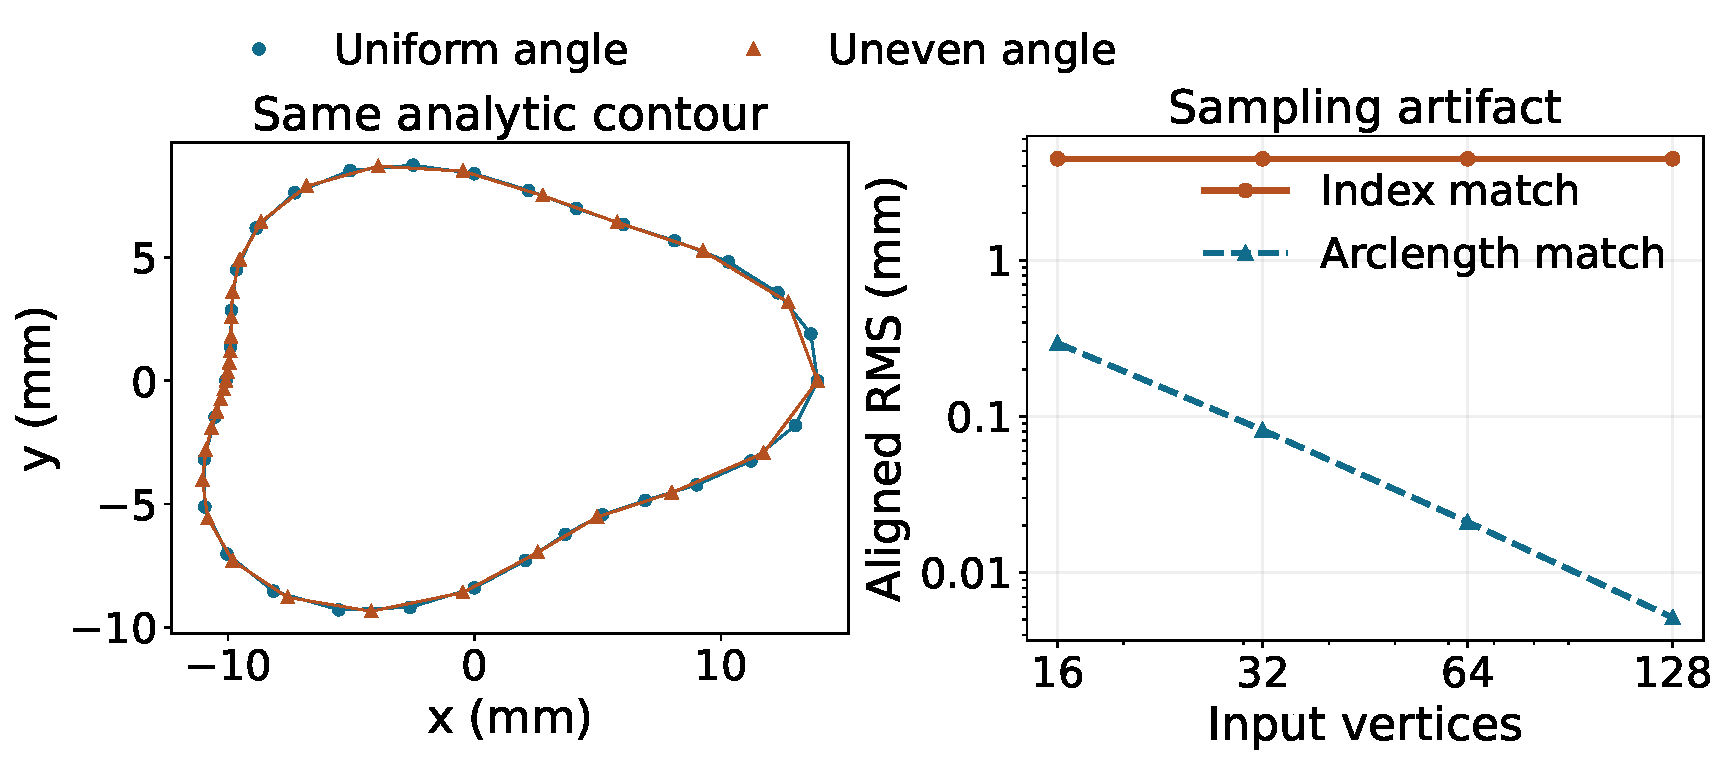
\includegraphics[width=.96\linewidth,height=.57\textheight,keepaspectratio]{sampling-artifact.pdf}\par\smallskip
{\small The same analytic curve is sampled with two angle conventions and a common start/direction. Refining input polygons reduces the RMS after resampling both to 128 equal polygonal-arclength points. Raw index matching remains mismatched. Output count is fixed; these are computed synthetic values.}
\end{minipage}\end{center}
\section{Degeneracies and retained geometric differences}
\hypertarget{note-degeneracies-and-retained-geometric-differences}{}\label{note:degeneracies-and-retained-geometric-differences}
{\small \href{slides.html\#frame=zero-length-edges-and-zero-spread\&step=1}{Slides for this section}}\par
Begin with a known identity rather than a complicated dataset. Comparing an array with itself should give zero RMS. Translating or properly rotating an array should leave its best rigid residual near zero when indices still correspond. Multiplying every coordinate by a positive factor changes a size-preserving comparison in physical units; it should not mysteriously disappear. Applying a reflection to an asymmetric configuration should generally leave a residual when only proper rotations are permitted. Symmetric objects can be special cases, which is why the test geometry must be named.

The code validates finite arrays, compatible dimensions and bounded control counts. Resampling rejects repeated adjacent vertices, including a duplicated closing endpoint, because those produce zero-length interpolation intervals. These checks prevent undefined calculations; they do not screen for every geometric defect. A self-intersecting polygon can still pass these numerical checks; validity as an anatomical boundary requires a separate geometric criterion.

Numerical tests should answer a stated question. A rotation determinant tests the allowed transformation. An RMS residual tests the fit to current correspondences. An input-refinement sequence tests sensitivity to polygon resolution. None substitutes for the others. A discrepancy becomes useful evidence when the changed assumption is identifiable.

If $Y=aX$ for a centered nondegenerate shape with $a>0$, the unscaled rigid residual cannot generally vanish when $a\ne1$. For an already matched orientation,
\[
 d_{\rm RMS}(X,aX)=|1-a|\sqrt{\frac1n\sum_j\|x_j\|^2}.
\]
Reflection also generally leaves a residual when the curve is asymmetric and only $SO(2)$ is allowed. Symmetries can make an optimizer nonunique; an attained minimum does not imply a unique anatomical correspondence.
\Needspace{10\baselineskip}

\section{Correspondence and the meaning of a residual}
\hypertarget{note-correspondence-and-the-meaning-of-a-residual}{}\label{note:correspondence-and-the-meaning-of-a-residual}
{\small \href{slides.html\#frame=residual-components\&step=1}{Slides for this section}}\par
Explain what remains unresolved. Arclength fractions are boundary positions, not validated anatomical landmarks. A planar curve misses three-dimensional structure. A local discrepancy might reflect segmentation, pose fitting, true morphology or an acquisition-plane difference. Full diffeomorphic registration introduces additional geometric structure and optimization beyond the present rigid fit.

Equal arclength is a representation convention rather than a landmark-identification procedure. It retains a chosen start and traversal direction, and it can only interpolate the supplied polygon. A residual after alignment can contain acquisition-plane differences, segmentation error, unresolved curvature or genuine shape variation. These sources are not separated by rigid fitting alone.
\bigskip
\section*{Exercises}
\par\noindent\begin{minipage}{\linewidth}
\subsection*{A13-1. Audit a translation}
New formative practice; 10 feedback points. Coordinates are in mm. X =\allowbreak{} [(0,0),(4,0),(0,2)] and Y =\allowbreak{} X +\allowbreak{} (-3,4).

\textbf{a} Compute both vertex centroids and the raw RMS discrepancy.

\end{minipage}\par\medskip
\textbf{b} Give the translation that maps Y to X and the resulting RMS.

\textbf{c} Explain why these vertex centroids need not be physical centers of mass, and name missing information for that claim.

\par\noindent\begin{minipage}{\linewidth}
\subsection*{A13-2. Declare a transformation}
X =\allowbreak{} [(0,0),(3,0),(0,1)]. A row-vector matrix R =\allowbreak{} [[0,-1],[1,0]] is supplied. New practice; 10 feedback points.

\textbf{a} Compute X R, state its rotation direction in the plane, and calculate det(R).

\end{minipage}\par\medskip
\textbf{b} Compare the longest pairwise length of X with that of 2X. Can a rigid motion make corresponding arrays identical?

\textbf{c} The matrix F =\allowbreak{} [[-1,0],[0,1]] maps X to a mirror image. State its determinant and explain whether the lesson allows it.

\par\noindent\begin{minipage}{\linewidth}
\subsection*{A13-3. Resample a rectangle}
Use ordered vertices [(0,0),(4,0),(4,2),(0,2)] mm, with the final edge closing to the first. New practice; 10 feedback points.

\textbf{a} Compute perimeter and the four targets for uniform arclength sampling with n =\allowbreak{} 4.

\end{minipage}\par\medskip
\textbf{b} Give the four resampled coordinates in traversal order.

\textbf{c} Would increasing the number of interpolated points recover a curved boundary that the rectangle had failed to capture? Explain.

\par\noindent\begin{minipage}{\linewidth}
\subsection*{A13-4. Diagnose a plausible overlay}
A report states: two 64-point contours have aligned RMS 0.2 mm, therefore their anatomy is identical. It omits units of the input, sampling rules and permitted transformations. New practice; 10 feedback points.

\textbf{a} Identify three missing specifications needed to interpret the reported number.

\end{minipage}\par\medskip
\textbf{b} Propose one controlled implementation check with a predicted result and one independent source of evidence for anatomical correspondence.

\textbf{c} Rewrite the claim with a defensible scope while preserving the reported result.

\section*{References}
\noindent\begin{minipage}{\linewidth}
Zan Ahmad, Advanced Topics in Computational Cardiology syllabus, Fall 2024. PDF pages 1--2.

\end{minipage}\par\medskip
\noindent\begin{minipage}{\linewidth}
Ahmad et al., A computational pipeline for clustering left atrial appendage morphology via elastic shape analysis, Computers in Biology and Medicine 196 (2025), 110905. PDF pages 2--4, methods: geometric representation, elastic path energy and relaxed matching.

\end{minipage}\par\medskip
\end{document}
